%!TEX root = Main.tex
\section{Implementation}
The following chapter seeks to explain the implementation of the mini project.

\subsection{Overall Design}
The full system is comprised of one or two PCs and two TelosB motes configured as a receiver and a sender. The system can be describes as seen in figure \ref{FullSystem}. 
\begin{figure}[H]
	\centering
	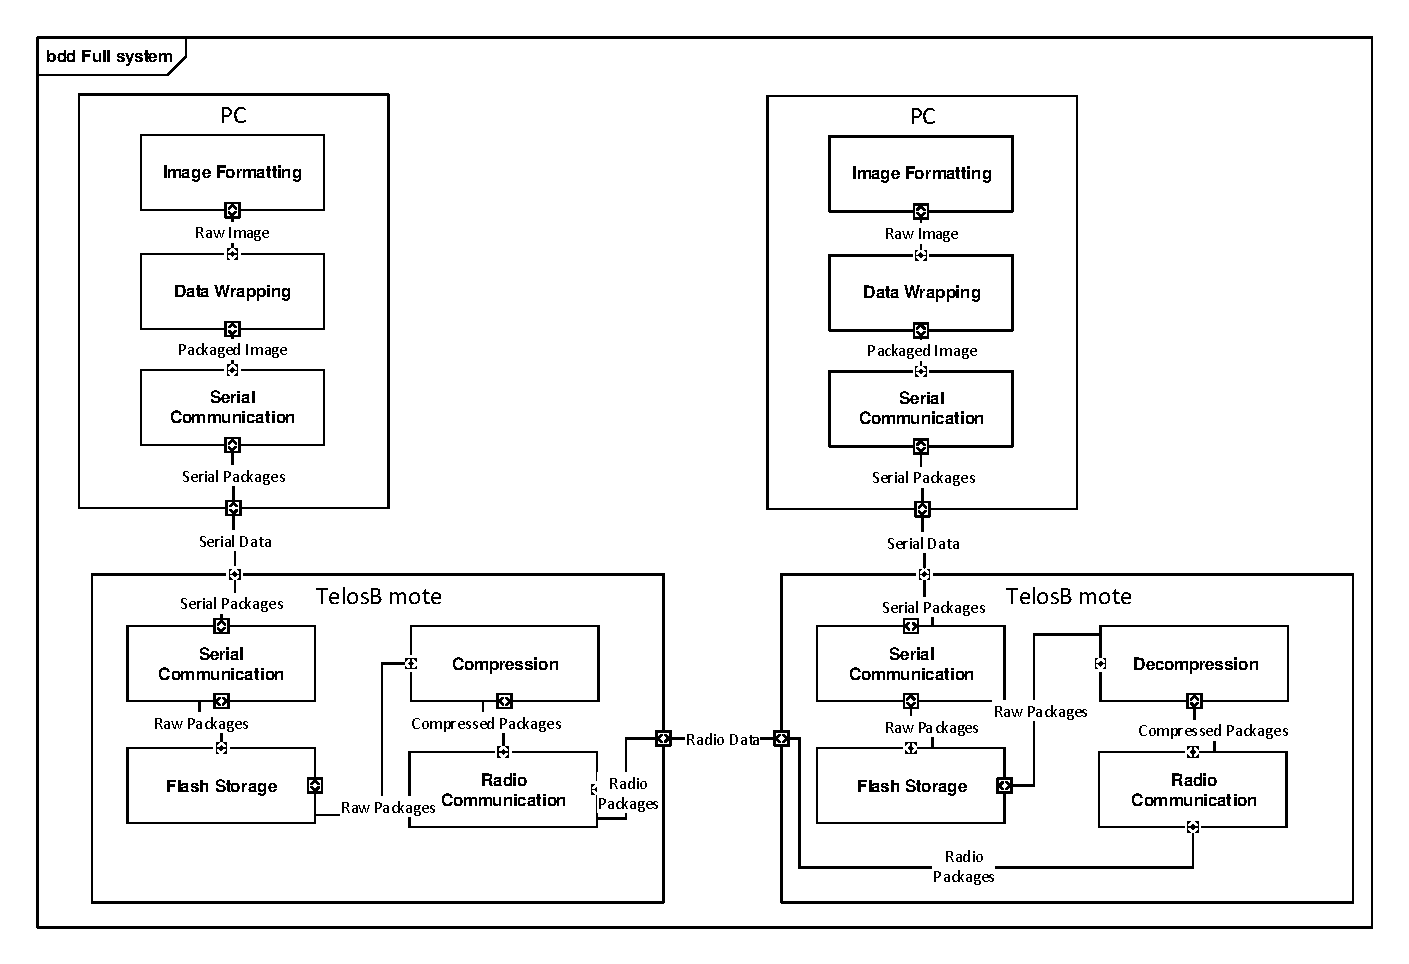
\includegraphics[width=1\textwidth]{FullSystem}
	\caption{Full System Diagram.}
	\label{FullSystem}
\end{figure}
The PC software has three responsibilities. It takes an image and converts it to a binary file. This file is then wrapped into an array and prepared such that it can be transmitted to the TelosB mote. The transmission is handled by the Serial Communication block and can be seen in the section \ref{sec:Serial-Communication}.

The TelosB motes are either configured as sender or receiver.  The sender has the responsibility of getting an image from the PC and transmitting it over the radio to the receiver mote. The receiver has the responsibility to receive the image from radio and transmitting it to the PC.

The Serial Communication block of the TelosB mote interacts with the PC's Serial Communication block as can be read in section \ref{sec:Serial-Communication}. 
The Radio Communication block interacts with other TelosB motes as can be read in section \ref{sec:Radio-Block}. 
Lastly the Compression block has entails the compression and decompression of the image data. 
This is explained in the section \ref{sec:Compression-block}.

\subsection{Serial Communication}
\label{sec:Serial-Communication}
The serial communication is responsible for the transfer of data to and from the TelosB. A header file is available to both the PC software and the TelosB program. It contains a series of defines that are used for the communication messages. The defines can be found in table \ref{definetable}.
\begin{table}[H]
\centering
    \begin{tabular}{lll}
    \hline
    Name                  & Val & Description                                               \\ \hline
    \rowcolor{gr}
    TRANSFER\_TO\_TELOS   & 1     & Used to tell the TelosB to prepare to receive the image. \\ %\hline
    TRANSFER\_OK          & 2     & Used to tell the PC that the transfer was ok.             \\ %\hline
    \rowcolor{gr}
    TRANSFER\_FAIL        & 3     & Used to tell the PC that the transfer failed.             \\ %\hline
    TRANSFER\_READY       & 4     & Used to tell the PC that the transfer can be initiated.   \\ %\hline
    \rowcolor{gr}
    TRANSFER\_FROM\_TELOS & 5     & Used to tell the TelosB to transfer the image to the PC.  \\ %\hline
    TRANSFER\_DONE        & 6     & Used to tell the PC that the image transfer is done.      \\ \hline
    \end{tabular}
    \caption{Defines for serial communication.}
    \label{definetable}
\end{table}

Using these defines and the TinyOS struct of \texttt{message\_t}, the PC and TelosB mote can exchange information. 
The sequence for transferring data to the TelosB can be found in figure \ref{transfertotelos}. 
Likewise the sequence for transferring data from the TelosB to the PC can be found in figure \ref{transferfromtelos}.

\begin{figure}[H]
	\centering
	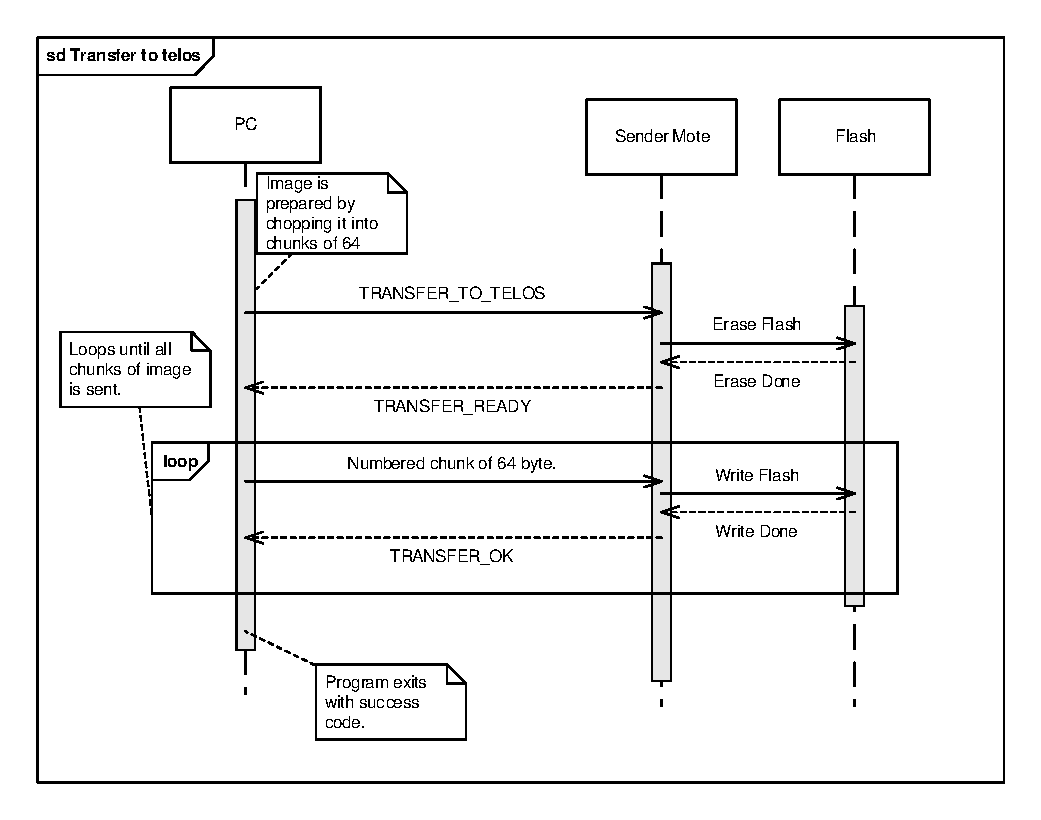
\includegraphics[width=0.8\textwidth]{PCtoTelosb}
	\caption{Transfer to TelosB sequence diagram.}
	\label{transfertotelos}
\end{figure}

The serial communication is initiated by the PC. 
The \texttt{TRANSFER\_OK} signal is used when transferring to the TelosB as the PC is faster than the TelosB. 
It also ensures that the TelosB is ready to receive. 
The TelosB has to use clock cycles to read and write to memory. 
When transferring to the PC it is assumed that the PC is ready before the TelosB starts sending. 
The PC software starts reconstructing the image to a binary file when the \texttt{TRANSFER\_DONE} is received. 
The binary file is loaded in Matlab and the image is reconstructed for human viewing.
\begin{figure}[H]
	\centering
	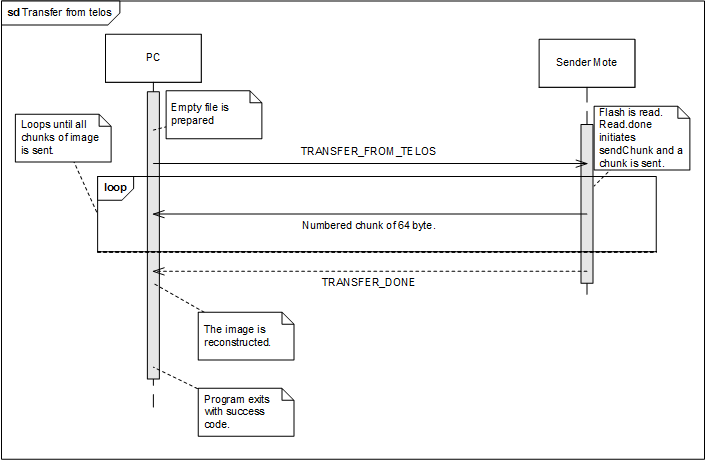
\includegraphics[width=0.8\textwidth]{PCfromTelosb}
	\caption{Transfer from TelosB sequence diagram.}
	\label{transferfromtelos}
\end{figure}
The PC software is implemented in Matlab and Java using image processing tools and the TinyOS example project "TestSerial". 
The TelosB software is based on the code used in multiple examples ranging from "BlockStorage" to "TestSerial". 



\subsection{Radio Block}
\label{sec:Radio-Block}





\subsection{Compression block}
\label{sec:Compression-block}

The compression blocks have a common interface: 

\begin{itemize}
    \item \texttt{uint16\_t Compress(uint8\_t* in, uint8\_t* out)}
    \item \texttt{void Decompress(uint8\_t *in, uint8\_t *out)}
\end{itemize}

This interface allows the different implementation to be accessed with the same code -- only specifying the desired block.

The \texttt{Compress(...)} method will take 1024 bytes in its first parameter, and return the compressed data in its second parameter, and return the size of the compression as return output.

The \texttt{Decompress(...)} method will, too, take the input as the first parameter and output as second parameter. 
The \texttt{Decompress(...)} method already knows how big the input is, and the output will always 1024 bytes.

\subsubsection{One Bit Compression}
The One Bit Compression's \texttt{Compress(...)} method will split the input data up in chunks of 8 bytes at a time, and for each byte AND \texttt{0xFE} onto it (resulting in the last bit being 0, and leave the rest untouched), and OR one bit from the last byte unto its own last bit.
Then the modified bytes will be added to the output parameter.
This will be done for all 128 chunks of bytes (8 bytes pr. chunk).
Lastly it will return the size of the output parameter.
This can be seen on Figure \ref{fig:1BitCompressingAlgo}.

\begin{figure}[htbp]
    \centering
    \begin{subfigure}[t]{0.3\textwidth}\tightdisplaymath
        \centerline{
        \xymatrix@ = 2pt{
            a   & a & a & a & a & a & a & a \\
            b   & b & b & b & b & b & b & b \\
            c   & c & c & c & c & c & c & c \\
            d   & d & d & d & d & d & d & d \\
            e   & e & e & e & e & e & e & e \\
            f   & f & f & f & f & f & f & f \\
            g   & g & g & g & g & g & g & g \\
            h   & h & h & h & h & h & h & h }}
        \caption{8 uncompressed bytes.}
    \end{subfigure}
    \begin{subfigure}[t]{0.3\textwidth}\tightdisplaymath
        \centerline{
        \xymatrix@=2pt{
            a   & a & a & a & a & a & a & \_ \\
            b   & b & b & b & b & b & b & \_ \\
            c   & c & c & c & c & c & c & \_ \\
            d   & d & d & d & d & d & d & \_ \\
            e   & e & e & e & e & e & e & \_ \\
            f   & f & f & f & f & f & f & \_ \\
            g   & g & g & g & g & g & g & \_ \\
            h \ar[uuuuuuurrrrrrr]   & h\ar[uuuuuurrrrrr]    & h \ar[uuuuurrrrr]& h \ar[uuuurrrr] & h \ar[uuurrr] & h \ar[uurr] & h \ar[ur] & \_ }}
            \caption{Mapping from 8 to 7 bytes.}
    \end{subfigure}
    \begin{subfigure}[t]{0.3\textwidth}\tightdisplaymath
        \centerline{
        \xymatrix@ = 1pt{
            a   & a & a & a & a & a & a & h \\
            b   & b & b & b & b & b & b & h \\
            c   & c & c & c & c & c & c & h \\
            d   & d & d & d & d & d & d & h \\
            e   & e & e & e & e & e & e & h \\
            f   & f & f & f & f & f & f & h \\
            g   & g & g & g & g & g & g & h }}
        \caption{7 compressed bytes.}
    \end{subfigure}%
    \caption{One bit compression algorithm.}
    \label{fig:1BitCompressingAlgo}
\end{figure}

The One Bit Compression's \texttt{Decompress(...)} is the inverse operation of the \texttt{Compress(...)} method.
For each chunk of seven bytes it will, for each byte, AND \texttt{0xFE} and store them in the output parameter. 
Then it will look at the last bit for the seven (unmodified) input bytes and shift each of them into a new byte, and store it after the seven modified bytes in the output parameter.





\subsubsection{Two Bit Compression}
The Two Bit Compression's \texttt{Compress(...)} method is similar to the One Bit Compression's \texttt{Compress(...)}.
The difference is, it will split the input data up in chunks of 4 bytes at a time, and for each byte AND \texttt{0xFC} onto it (resulting in the last two bits being 0, and leave the rest untouched), and OR two bits from the last byte unto its own last two bits.
This can be seen on Figure \ref{fig:2BitCompressingAlgo}.

\begin{figure}[htbp]
    \centering
    \begin{subfigure}[t]{0.3\textwidth}\tightdisplaymath
        \centerline{
        \xymatrix@ = 2pt{
            a   & a & a & a & a & a & a & a \\
            b   & b & b & b & b & b & b & b \\
            c   & c & c & c & c & c & c & c \\
            d   & d & d & d & d & d & d & d }}
        
        \caption{4 uncompressed bytes.}
    \end{subfigure}
    \begin{subfigure}[t]{0.3\textwidth}\tightdisplaymath
        \centerline{
        \xymatrix@=2pt{
            a   & a & a & a & a & a & \_ & \_ \\
            b   & b & b & b & b & b & \_ & \_ \\
            c   & c & c & c & c & c & \_ & \_ \\
            d \ar[uuurrrrrr]    & d\ar[uuurrrrrr]   & d\ar[uurrrr]  & d\ar[uurrrr]  & d\ar[urr] & d\ar[urr] & \_ & \_ }}
        
        \caption{Mapping from 4 to 3 bytes.}
    \end{subfigure}
    \begin{subfigure}[t]{0.3\textwidth}\tightdisplaymath
        \centerline{
        \xymatrix@ = 1pt{
            a   & a & a & a & a & a & d & d \\
            b   & b & b & b & b & b & d & d \\
            c   & c & c & c & c & c & d & d }}
        \caption{3 compressed bytes.}
    \end{subfigure}%
    \caption{Two bit compression algorithm.}
    \label{fig:2BitCompressingAlgo}
\end{figure}

Like \texttt{Compress(...)} method is similar, so is the \texttt{Decompress(...)} method. 
For each chunk of 3 bytes it will, for each byte, AND \texttt{0xFC} and store them in the output parameter. 
Then it will look at the last two bits for the three (unmodified) input bytes and shift each of them into a new byte, and store it after the three modified bytes in the output parameter.




\subsubsection{Four Bit Compression}

The Four Bit Compression's \texttt{Compress(...)} method than both the One- and Two Bit Compression's \texttt{Compress(...)}.
The difference is, it will split the input data up in chunks of 2 bytes at a time,  AND \texttt{0xF0} onto it (resulting in the last four bits being 0, and leave the rest untouched), and OR the first four  bits from the second byte unto the first byte's own last four bits.
This can be seen on Figure \ref{fig:4BitCompressingAlgo}.


\begin{figure}[htbp]
    \centering
    \begin{subfigure}[t]{0.3\textwidth}\tightdisplaymath
        \centerline{
        \xymatrix@ = 2pt{
            a   & a & a & a & a & a & a & a \\
            b   & b & b & b & b & b & b & b }}
        
        \caption{2 uncompressed bytes.}
    \end{subfigure}
    \begin{subfigure}[t]{0.3\textwidth}\tightdisplaymath
        \centerline{
        \xymatrix@=1pt{
            a   & a & a & a & \_ & \_ & \_ & \_ \\
            b \ar[urrrr] & b\ar[urrrr] & b\ar[urrrr] & b \ar[urrrr] & \_ & \_ & \_ & \_ }}
        
        \caption{Mapping from 2 to 1 byte.}
    \end{subfigure}
    \begin{subfigure}[t]{0.3\textwidth}\tightdisplaymath
        \centerline{
        \xymatrix@ = 1pt{
            a   & a & a & a & b & b & b & b }}
        \caption{1 compressed byte.}
    \end{subfigure}
    \caption{Four bit compression algorithm.}
    \label{fig:4BitCompressingAlgo}
\end{figure}

The \texttt{Decompress(...)} method will AND \texttt{0xF0} on each byte and store them in the output parameter. 
Then it will shift at the last four bits of the unmodified input byte into a new byte, and store it after the previous modified byte in the output parameter.